\chapter{Data}\label{ch:data}

This chapter identifies the ECG sources, explains how the real signals are
cleaned, and shows how examples enter model fitting, validation, and the
temporal test. Keeping these roles separate prevents healthy data or test
labels from being used in the wrong part of the study.

\section{Data Sources and Roles}

The study uses two public PhysioNet databases. The MIT--BIH Normal Sinus Rhythm
Database (NSRDB) supplies only healthy ECG for the autoencoder. The MIT--BIH
Arrhythmia Database (MITDB) supplies labeled normal and abnormal beats for the
detector, subtype classifier, and final temporal evaluation
\cite{goldberger2000physionet,nsrdb,mitdb}.

\begin{table}[H]
\centering
\small
\caption{Data sources and their strictly separated roles.}
\label{tab:data-source-role}
\begin{tabular}{@{}>{\raggedright\arraybackslash}p{2.6cm}>{\raggedright\arraybackslash}p{3.8cm}>{\raggedright\arraybackslash}p{4.8cm}@{}}
\toprule
Source & Available data & Use in this study\\
\midrule
\makecell[l]{MIT--BIH\\Normal Sinus\\Rhythm DB\\(NSRDB)} &
18 real long-term ECG recordings from five men aged 26--45 and 13 women aged
20--50, with no significant arrhythmias; two stored channels named ECG1 and
ECG2; 128 Hz; approximately 23--26 hours per record \cite{nsrdb}. &
The complete first stored ECG channel from every record is processed. Fifteen
subjects fit the normal-only autoencoder and three different subjects validate
it and determine the normal residual threshold.\\
\addlinespace
\makecell[l]{MIT--BIH\\Arrhythmia DB\\(MITDB)} &
48 approximately 30-minute, two-channel ambulatory ECG records from 47
subjects (25 men aged 32--89 and 22 women aged 23--89), sampled at 360 Hz,
with expert beat and rhythm annotations \cite{mitdb,moody2001impact}. &
Only the 46 records containing MLII are eligible. Their earlier 80\% supplies
supervised development and their final 20\% supplies the temporal test. These
records represent 45 subject clusters because records 201 and 202 belong to
one person.\\
\bottomrule
\end{tabular}
\end{table}

Figure~\ref{fig:data-source-overview} gives the same information as a flow
diagram. In short, NSRDB contributes only healthy windows for the frozen
autoencoder, while MITDB contributes MLII beats for supervised development and
the final temporal test.

\begin{figure}[H]
\centering
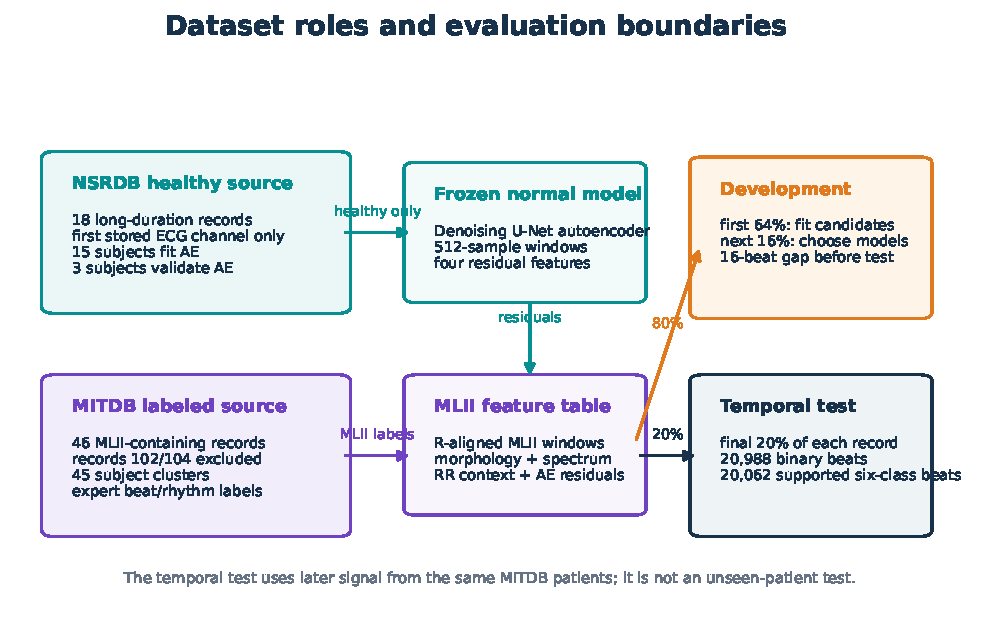
\includegraphics[width=.98\textwidth]{pic/generated/dataset_role_overview.pdf}
\caption{Dataset roles and evaluation boundaries. The healthy NSRDB channel
creates the frozen normal model. MITDB MLII creates the supervised feature table
and is split chronologically into development and temporal-test regions.}
\label{fig:data-source-overview}
\end{figure}

\textbf{Why NSRDB is used for healthy training.}
NSRDB contains real long-duration ECG from subjects reported to have no
significant arrhythmias. This matches the autoencoder idea: the network sees
normal structure but receives no arrhythmia examples or labels. All 18 subjects
and their complete recordings enter the cleaning process, giving 437.49 hours
of source ECG. Complete recordings also expose the model to normal within-day
variation instead of a short selected excerpt.

\textbf{Exactly one channel is used.}
NSRDB headers call the two waveforms ECG1 and ECG2; they do not identify either
as a standard anatomical lead. This study therefore selects the first stored
channel consistently and describes it as the \emph{first NSRDB ECG channel}.
It is not renamed Lead II. The second channel never enters autoencoder fitting,
validation, threshold estimation, or residual calculation.

The supervised branch uses MLII only. In the deployed placement, MLII is formed
from torso electrodes with the negative electrode near the right upper chest,
the positive electrode on the left lower chest or rib region, and a reference
electrode on the lower right torso. This modified Lead-II axis usually shows a
prominent QRS complex, making beat shape and RR timing clear \cite{mitdb}. The
loader selects MLII by its header name rather than assuming a channel number.
MLII is stored first in 45 eligible records; record 114 stores V5 first and
MLII second. Records 102 and 104 contain V5 and V2 but no MLII and are
excluded. Consequently, the detector, classifier, temporal test, and installed
replay all receive one MLII waveform.

The two model stages are one-channel systems, but the channel identities are
not falsely treated as identical: the autoencoder learns healthy structure
from the first NSRDB channel, while the supervised hierarchy operates on MLII.
This source difference is a limitation because the electrode placement for the
NSRDB channel is not documented.

\begin{figure}[H]
\centering
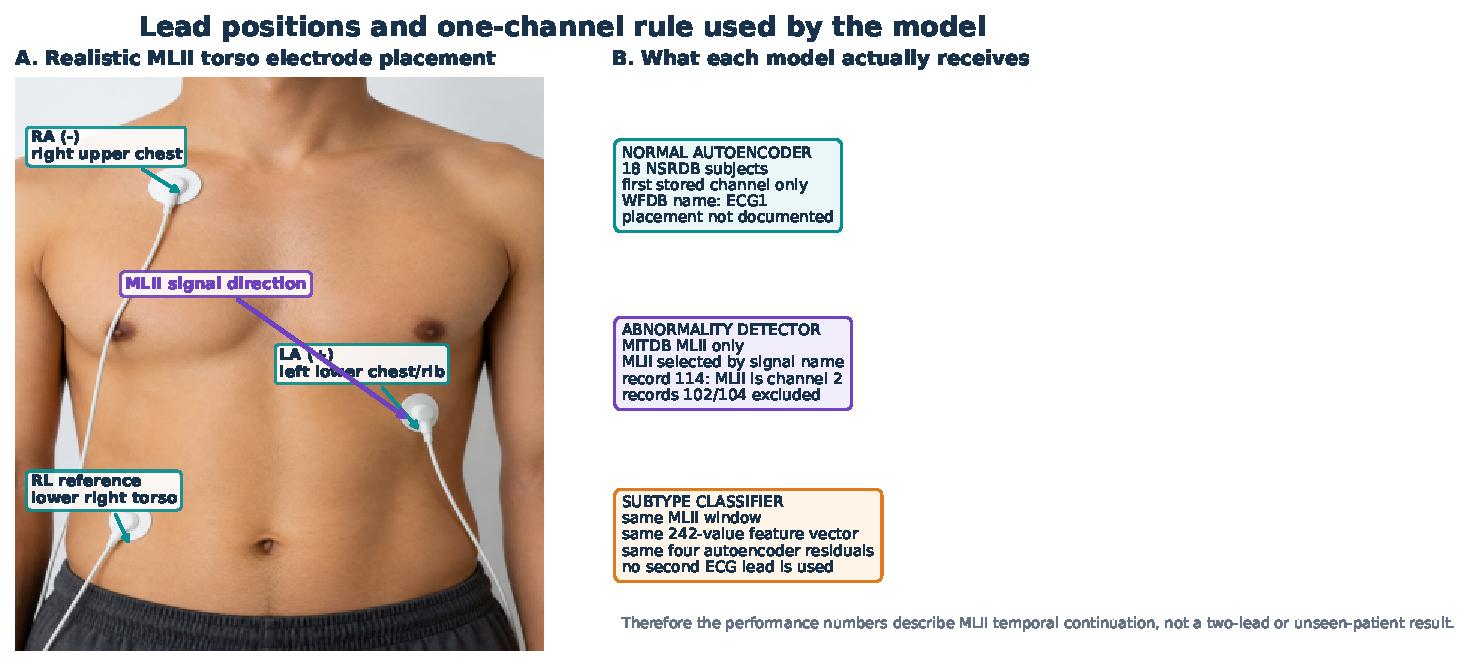
\includegraphics[width=.98\textwidth]{pic/generated/real_lead_positions.pdf}
\caption{Physical MLII placement and the exact one-channel rule. The normal
autoencoder uses only the first stored NSRDB ECG channel, whose anatomical
placement is unspecified. The supervised and deployed system uses only MLII:
negative electrode on the right upper chest, positive electrode on the left
lower chest/rib region, and reference electrode on the lower right torso.}
\label{fig:data-lead-positions}
\end{figure}

\textbf{Reference labels.}
MITDB expert annotations are mapped to the six project outputs as shown in
Table~\ref{tab:data-label-map}. AFib is determined from the rhythm annotation
around a beat; the other targets mainly use beat symbols.

\begin{table}[H]
\centering
\small
\caption{Mapping from MITDB expert annotations to project outputs.}
\label{tab:data-label-map}
\begin{tabular}{lll}
\toprule
Output & MITDB evidence & Interpretation\\
\midrule
N & N, e, j outside AFib/AFL & normal beat\\
PVC & V, E & ventricular premature or escape beat\\
PAC & A, a, J, S & supraventricular premature beat\\
LBBB & L & left bundle branch block beat\\
RBBB & R & right bundle branch block beat\\
AFib & normal-like beat inside AFIB/AFL rhythm & atrial fibrillation/flutter context\\
\bottomrule
\end{tabular}
\end{table}

Unsupported symbols remain abnormal in binary evaluation but are not forced
into a wrong subtype. The MLII cache contains 104,847 accepted beats: 63,130
normal and 41,717 abnormal. Of these, 100,159 have a supported six-class label.

\section{Data Cleaning}

Data cleaning converts two different raw ECG sources into the same numerical
input: one four-second signal with 512 samples. The cleaning rules are fixed
before evaluation and are reused after installation.
Figure~\ref{fig:data-cleaning-real} shows the full transformation for one
healthy NSRDB segment and one MITDB MLII beat.

\subsection{Cleaning Checklist}

The cleaning pipeline is easier to check as a list. Each item has one purpose
and one failure rule.

\begin{table}[H]
\centering
\small
\caption{Cleaning checklist applied before a signal can become a model input.}
\label{tab:data-cleaning-checklist}
\begin{tabular}{>{\raggedright\arraybackslash}p{2.6cm}>{\raggedright\arraybackslash}p{5.0cm}>{\raggedright\arraybackslash}p{4.3cm}}
\toprule
Step & What is done & Why it matters\\
\midrule
Required channel & NSRDB must provide ECG1; MITDB must provide MLII. Missing
required signals stop processing. & Prevents accidental use of ECG2, V5, V2, or
another non-matching lead.\\
\addlinespace
Sampling rate & NSRDB remains at 128 Hz. MITDB MLII is resampled from 360 Hz to
128 Hz with polyphase anti-aliasing. & Makes every four-second model window
exactly 512 samples.\\
\addlinespace
Band-pass filter & A fourth-order zero-phase Butterworth 0.5--50 Hz filter is
applied \cite{butterworth1930filter,virtanen2020scipy}. & Reduces baseline
movement and high-frequency noise without shifting the QRS complex.\\
\addlinespace
Amplitude standardisation & Each window is converted to approximately zero mean
and unit standard deviation. & Reduces gain differences while preserving the
relative P--QRS--T shape.\\
\addlinespace
Window quality check & Windows must be finite, non-flat, and have reasonable
variation. & Removes unusable or filter-edge examples before training or
scoring.\\
\bottomrule
\end{tabular}
\end{table}

\subsection{Window Construction}

The autoencoder and supervised hierarchy build windows in different ways, but
the final array shape is the same. The autoencoder receives consecutive,
non-overlapping four-second windows from the first stored NSRDB channel. The
supervised MLII windows are centred on a beat: 200 samples before the R peak
and 312 samples after it. During offline experiments, expert annotations give
the R-peak location for alignment and later scoring. During live use, detected
R peaks replace those annotations.

For samples $x_1,\ldots,x_n$ inside one prepared model window, amplitude
standardisation is
\begin{equation}
 z_i=\frac{x_i-\mu}{\sigma+10^{-8}},\qquad
 \mu=\frac{1}{n}\sum_{i=1}^{n}x_i.
\end{equation}
This operation is applied window by window, not once across an entire record.

\subsection{Cleaning Yield}

The healthy NSRDB recordings produce many candidate windows because complete
records are used instead of short excerpts. Across the 18 complete NSRDB
records, 393,744 candidate windows were formed. The quality checks kept 345,850
windows and rejected 47,894. These accepted windows were then split into
288,673 autoencoder fitting windows and 57,177 validation windows.

MITDB cleaning produces beat-centered MLII examples. The accepted MLII cache
contains 104,847 beats: 63,130 normal and 41,717 abnormal. Unsupported abnormal
symbols are still used for binary abnormality evaluation, but they are excluded
from six-class subtype scoring.

\subsection{Installed Use}

Installed use applies the same sampling rate, filter, standardisation,
512-sample window length, and feature order. Labels never enter a prediction.
The live backend waits until there is enough signal around a detected R peak
and enough RR context. It then feeds one prepared MLII window to the frozen
system. Neither supervised model is retrained during prediction.

\begin{figure}[H]
\centering
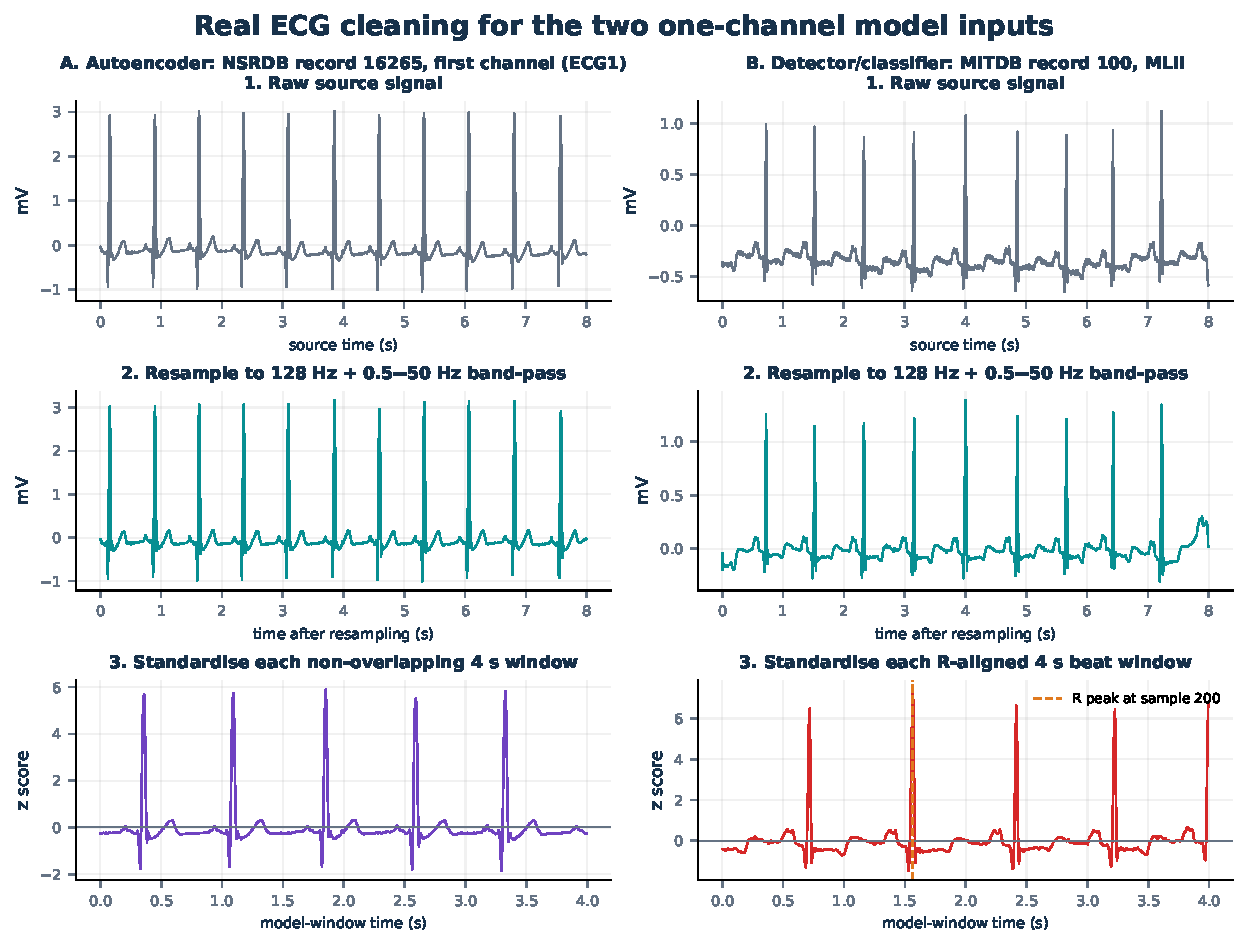
\includegraphics[width=.96\textwidth]{pic/generated/real_data_cleaning_pipeline.pdf}
\caption{Cleaning real ECG for the two roles. The healthy example is the first
channel of NSRDB record 16265. The unseen-use example is MLII from MITDB record
100. Both become one 512-sample input, but their documented channel identities
remain different.}
\label{fig:data-cleaning-real}
\end{figure}

\section{Data Preparation}

Data preparation decides which cleaned examples are allowed to fit a model,
which examples choose model settings, and which examples are held back for the
final temporal result. Figure~\ref{fig:data-feed-real} shows this flow from
raw source to frozen prediction.

\subsection{Prepared Objects}

After cleaning, the study keeps two kinds of prepared object:
\begin{itemize}
    \item \textbf{NSRDB window:} a healthy $[1,512]$ window from the first
    stored ECG channel. It has no arrhythmia label and is used only by the
    normal autoencoder.
    \item \textbf{MITDB beat:} an R-aligned MLII $[1,512]$ window with record
    identity, binary normal/abnormal truth, supported subtype truth when
    available, and RR timing context.
\end{itemize}

The autoencoder input tensor has shape $[B,1,512]$. The supervised detector and
subtype classifier do not receive raw samples alone. Each MITDB beat is
converted into the same 242-value MLII feature vector:
\[
\begin{aligned}
242\ \text{values}={}&230\ \text{morphology, spectrum, statistics, and base-RR values}\\
&+8\ \text{causal RR-history values}\\
&+4\ \text{autoencoder residual values}.
\end{aligned}
\]
The subtype model is fitted only on the five supported abnormal classes: PVC,
PAC, LBBB, RBBB, and AFib.

\subsection{Splits}

The autoencoder split is subject-disjoint. A seeded split assigns 15 complete
NSRDB records to fitting and three different records (16420, 16483, and 16795)
to validation. This produces 288,673 fitting windows and 57,177 validation
windows. Validation selects the checkpoint and estimates the normal residual
threshold. There is no separate healthy test because the autoencoder is frozen
before it contributes residual features to MITDB evaluation.

The MITDB split is chronological inside every eligible record:
\begin{itemize}
    \item the first 64\% fits candidate supervised models;
    \item the next 16\% selects the model structures and abnormal-probability
    threshold;
    \item a 16-beat gap is removed before the test boundary; and
    \item the final 20\% evaluates the completed frozen hierarchy.
\end{itemize}
This is a temporal continuation test from known patients. It is stronger than a
shuffled-beat split, but it is not an unseen-patient test.

\subsection{Exact Model Allocation}
\begin{table}[H]
\centering
\small
\caption{Training, validation, and temporal-test data supplied to each model.}
\label{tab:data-model-allocation}
\begin{tabular}{>{\raggedright\arraybackslash}p{2.3cm}>{\raggedright\arraybackslash}p{3.0cm}>{\raggedright\arraybackslash}p{3.0cm}>{\raggedright\arraybackslash}p{3.2cm}}
\toprule
Model & Candidate training & Validation & Final fitting and testing\\
\midrule
Autoencoder & 288,673 first-channel windows from 15 complete NSRDB records & 57,177 windows from 3 different complete NSRDB records & Frozen while every MLII test beat produces four residual features\\
\addlinespace
Abnormality detector & 66,344 MLII beats: 40,505 normal and 25,839 abnormal & 16,043 beats: 9,671 normal and 6,372 abnormal & Fitted on 83,123 development beats; tested on 20,988 temporal-test beats\\
\addlinespace
Subtype classifier & 22,864 supported abnormal MLII beats & 5,657 supported abnormal beats & Fitted on 28,784 supported abnormal beats; conditionally tested on 7,964 supported abnormal beats\\
\bottomrule
\end{tabular}
\end{table}

The supported six-output test contains 20,062 beats: 12,098 N, 1,527 PVC,
591 PAC, 1,482 LBBB, 1,383 RBBB, and 2,981 AFib. Another 926 unsupported
abnormal beats remain in binary testing but not six-class scoring.

\begin{figure}[H]
\centering
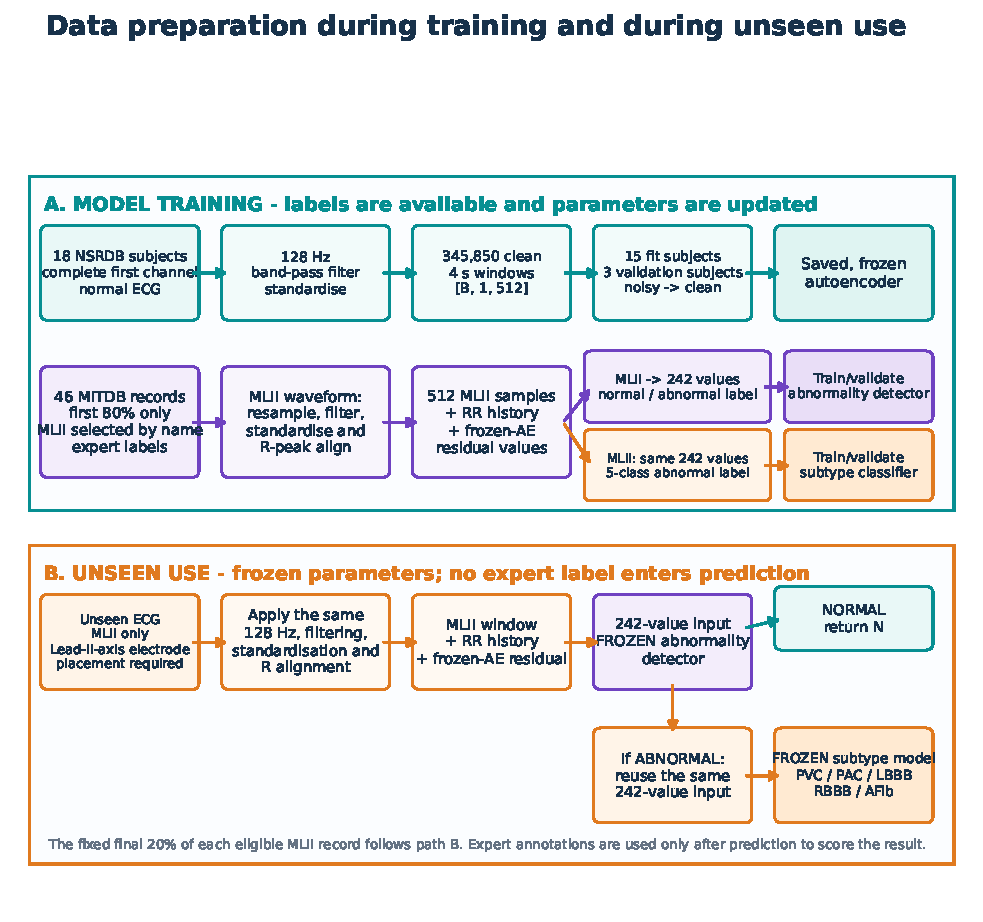
\includegraphics[width=.95\textwidth]{pic/generated/real_data_preparation_flow.pdf}
\caption{Data preparation during model development and use. Panel A separates
normal-only autoencoder development from labeled MLII development. Panel B
shows one new MLII signal passing through the frozen abnormality gate and then,
only when abnormal, the subtype classifier.}
\label{fig:data-feed-real}
\end{figure}

\subsection{Feeding the Frozen System}

During autoencoder fitting, Gaussian noise with standard deviation 0.03 is
added to each input while the clean NSRDB window remains the target. During
supervised fitting, record-and-class weights reduce domination by long records
and common classes. During prediction, one MLII window and its causal RR
history are converted into the same 242-value vector used in the temporal
experiment. A normal decision stops. An abnormal decision reuses that vector
for PVC, PAC, LBBB, RBBB, or AFib classification.
